%!TEX root= ../../../report.tex

\section{From the wheel to the leg} % (fold)
\label{sec:from_the_wheel_to_the_leg}
While the wheel is a young human invention meant to facilitate terrestrial motion, legged locomotion has been the result of millions of years of adaption of the species from aquatic to terrestrial fields.
Even though other forms of motion emerged during the same process, including limbless or rolling, the tetrapod and quadrupedal motion is the one that has proved the best performance in terrestrial displacement in relative velocity or jump length, for instance.

\subsection{The wheel in robotics} % (fold)
\label{sub:the_wheel_in_robotics}
Despite the facts above, it was the wheel the mean chosen to implement the ability to move around on the first mobile robots such as Walter's tortoises or the John Hopkins University robot Beast \cite{first_mobile_robot}, \cite{second_mobile_robot}.
This could be explained due to the fact that, as an artificial human creation, the modeling and control of the wheel could be fully mastered during its evolution process, easing its implementation in robotic platforms.
Some examples of this are shown in Figure \ref{fig:mobile_robots}, which depicts three different applications of wheeled robots.

The Rover "Spirit", in \ref{fig:mobile_rover}, is a good example of the possibilities and limits entailed by wheel-based locomotion.
It was successfully launched on Mars surface in 2004, which can be considered one of the most challenging and unpredictable environment a robot can be subject to, and it stayed active and operative until 2010.
However, the end of the mission came from the hand of the terrain. 
A very low-cohesion area of soil made the wheels of the device loose traction and eventually get trapped, preventing from recovering the control of the vehicle and bringing about the end of the mission.

Figure \ref{fig:mobile_mir} shows a MIR 100 robot, a state-of-the-art service robot designed for independent transportation and logistics in a dynamic and unpredictable environment..
As a service robot, it must fulfill strict safety standards and guarantee a secure interaction with users and other equipment while accomplishing its tasks.
Thanks to its wheels configuration, it can achieve an agile mobility, fast reaction capacity and a big load capacity.

The EMIEW 2, in \ref{fig:mobile_hitachi}, is an example of midpoint between wheeled and legged locomotion.
Although its motion relies on steering wheels, their placement at the end of two leg-like limbs provides with some of the advantages of bipedal motion, such as active suspension or impact absorption.

\begin{figure}[h]
\label{fig:mobile_robots}
	\centering
    \begin{subfigure}[b]{0.32\textwidth}
        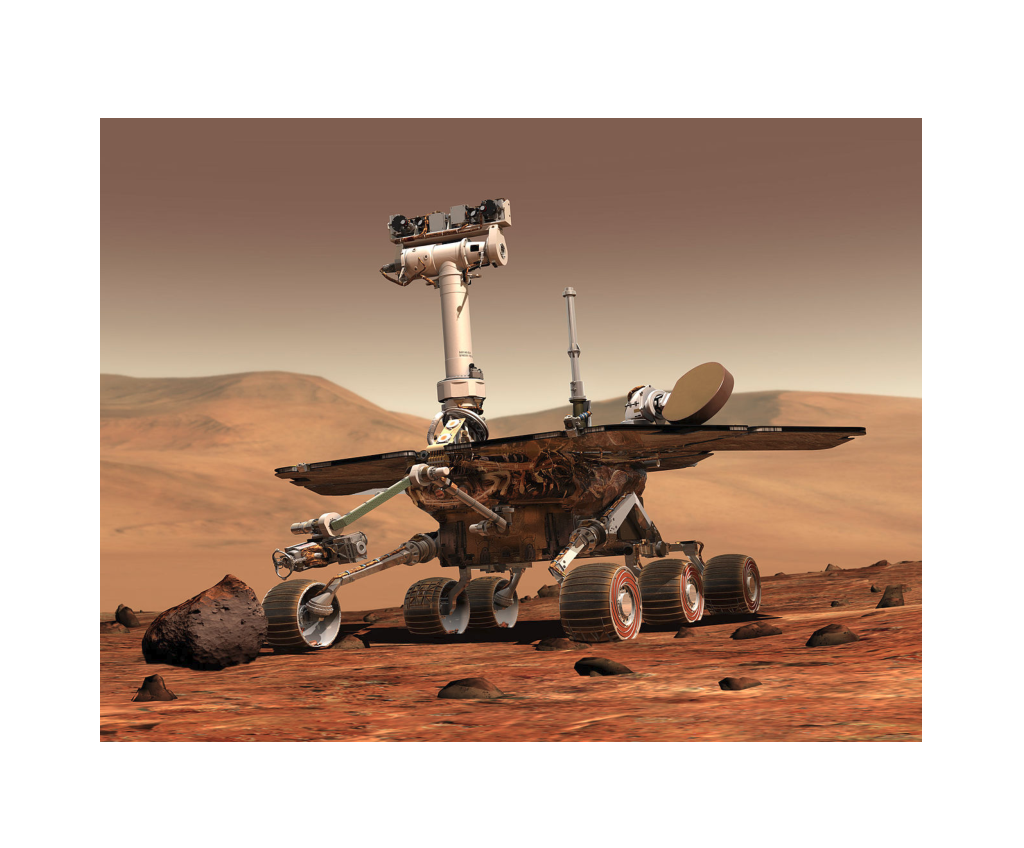
\includegraphics[width=\textwidth]{figures/mobile_rover.pdf}
        \caption{Mars Rover Spirit}
        \label{fig:mobile_rover}
    \end{subfigure}
    \centering
    \begin{subfigure}[b]{0.32\textwidth}
        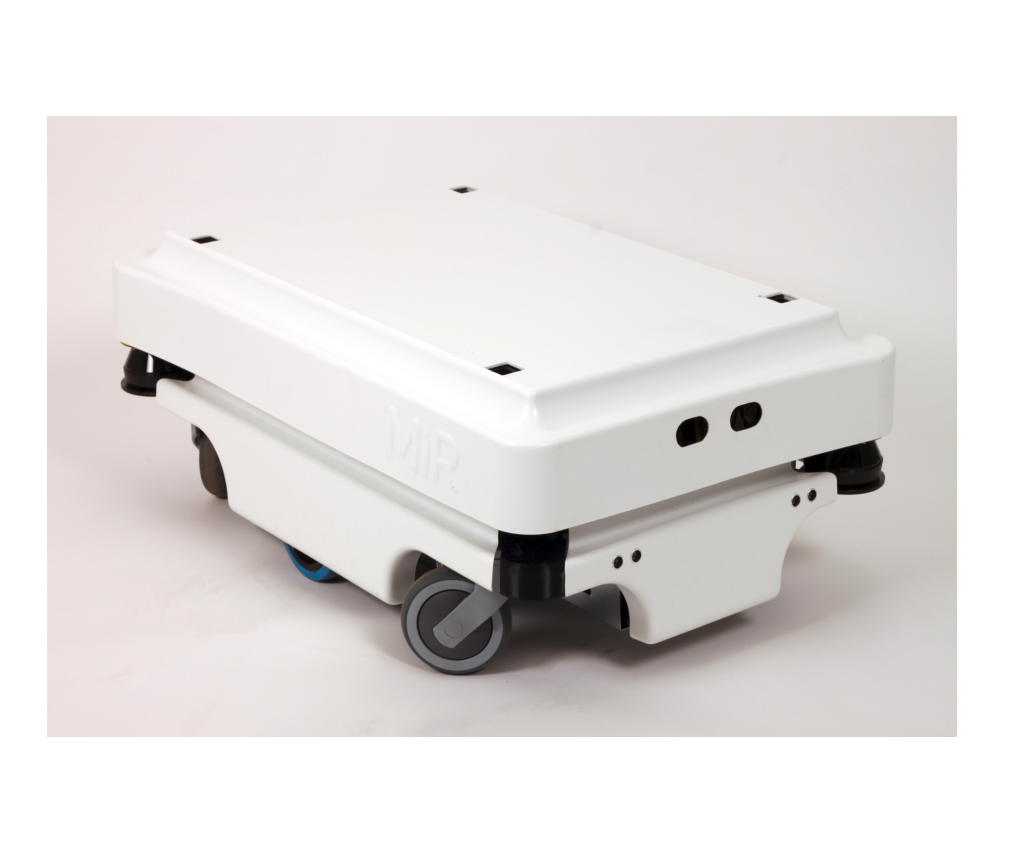
\includegraphics[width=\textwidth]{figures/mobile_mir.pdf}
        \caption{MIR 100 by MIR}
        \label{fig:mobile_mir}
    \end{subfigure}
    \centering
    \begin{subfigure}[b]{0.32\textwidth}
        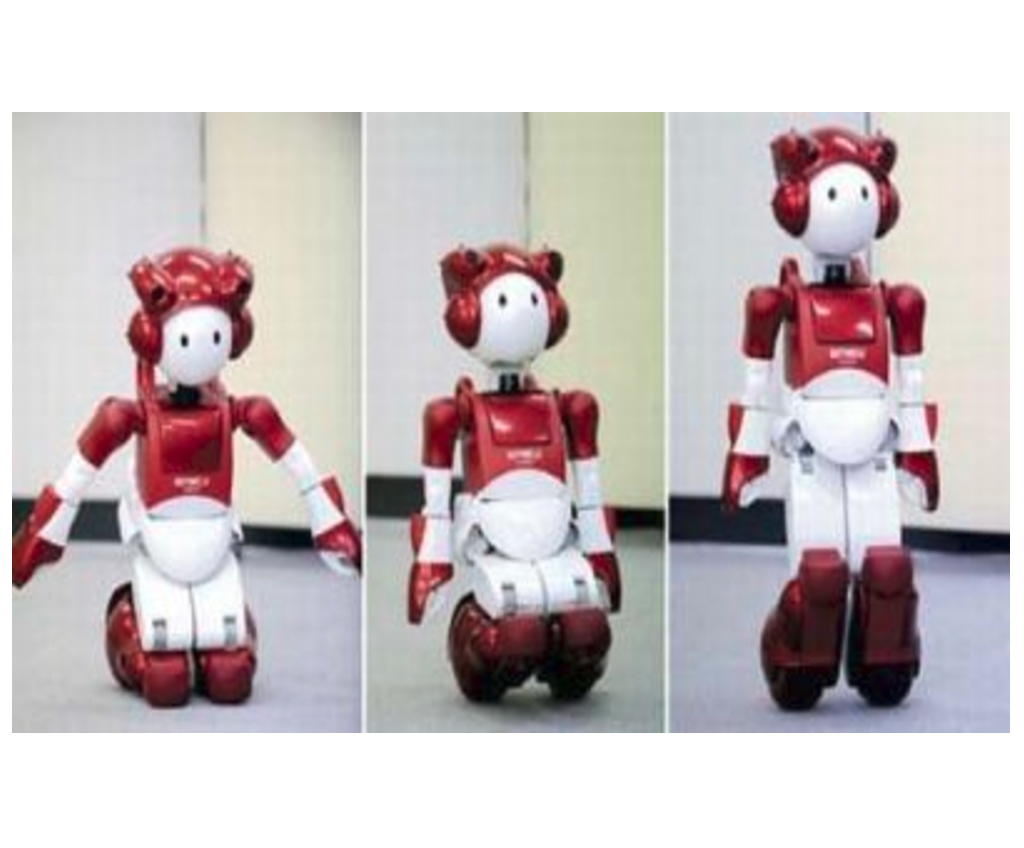
\includegraphics[width=\textwidth]{figures/mobile_hitachi.pdf}
        \caption{EMIEW2, by Hitachi}
        \label{fig:mobile_hitachi}
    \end{subfigure}
\end{figure}

% subsection the_wheel_in_robotics (end)

\subsection{Achieving legged motion} % (fold)
\label{sub:legged_motion_in_robotics}
In spite of the great successes attained in the field of wheeled-robotics, possible thanks to the development in engines and the increasing computing capacity of processors, mobile robots based on wheels have not been able to achieve performances in motion comparable to the ones found in nature.
Specially in uneven terrains, velocity, agility and efficiency are still problems under study.
Besides, the absence of wheels in nature as a result of darwinian evolution \cite{dawkins} ultimately led to questioning if they are truly the best mean to overcome the challenges that displacements in uneven, unknown surfaces yield for robots.

\begin{figure}[h]
\label{fig:mobile_robots}
	\centering
    \begin{subfigure}[b]{0.32\textwidth}
        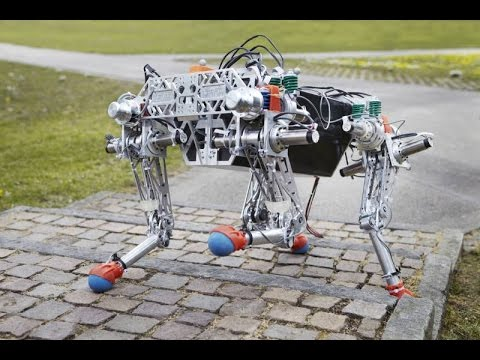
\includegraphics[width=\textwidth]{figures/starleth.jpg}
        \caption{STARLeth}
        \label{fig:mobile_rover}
    \end{subfigure}
    \centering
    \begin{subfigure}[b]{0.32\textwidth}
        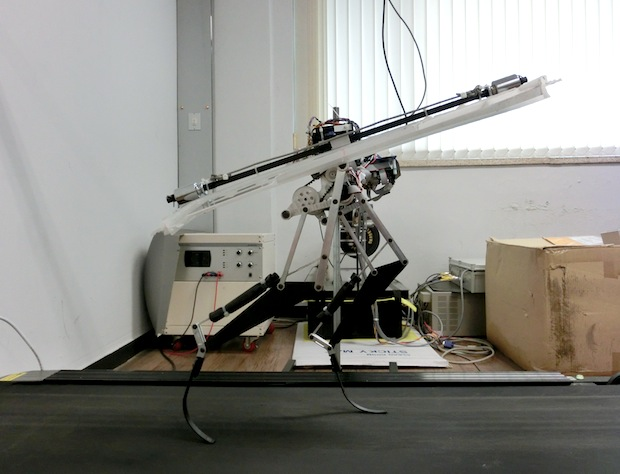
\includegraphics[width=\textwidth]{figures/biped_kaist.jpg}
        \caption{Raptor}
        \label{fig:mobile_mir}
    \end{subfigure}
    \centering
    \begin{subfigure}[b]{0.32\textwidth}
        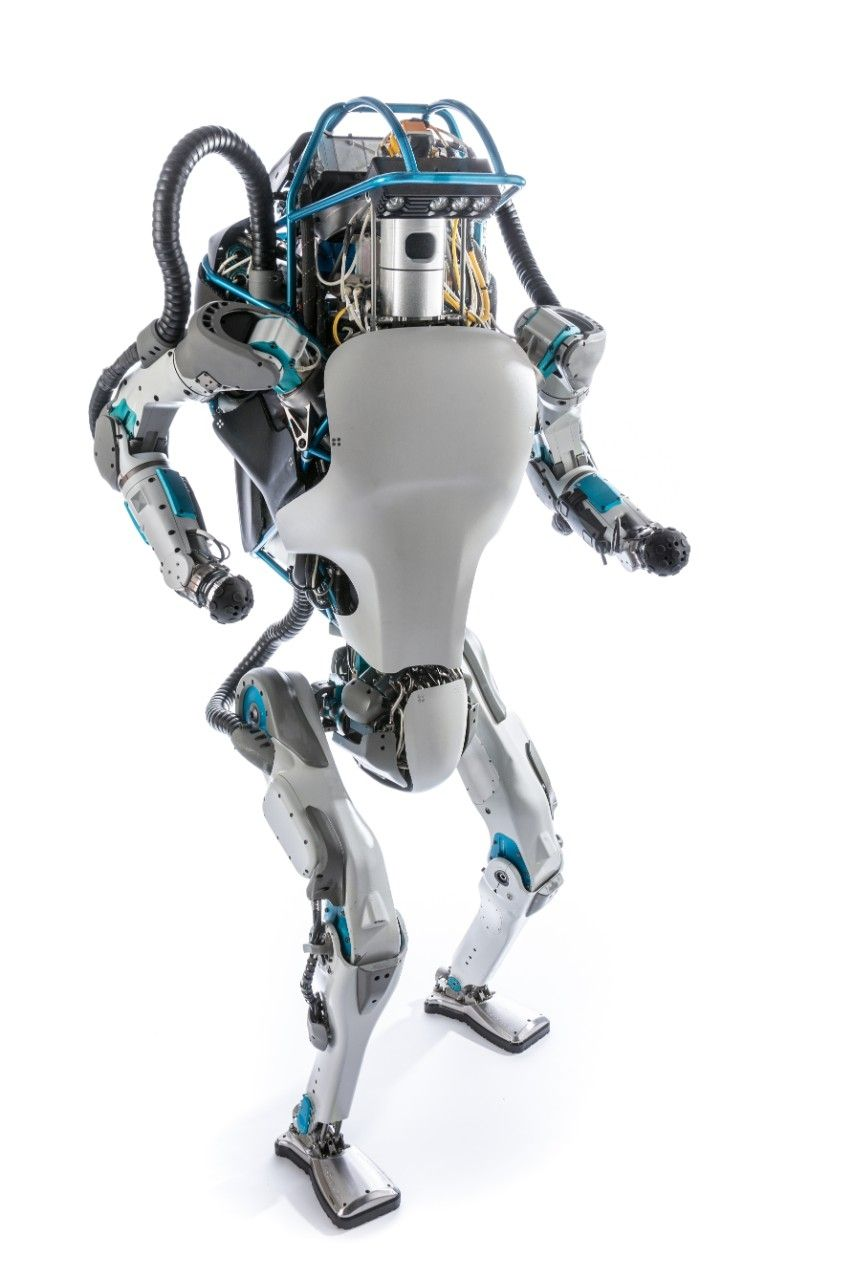
\includegraphics[width=\textwidth]{figures/biped_atlas.jpg}
        \caption{ATLAS}
        \label{fig:mobile_hitachi}
    \end{subfigure}
\end{figure}


% subsection legged_motion_in_robotics (end)





% section from_the_wheel_to_the_leg (end)